\documentclass[10pt,sigplan,authorversion=true]{acmart}
\settopmatter{printfolios=true,printccs=true,printacmref=true}

\bibliographystyle{ACM-Reference-Format}
\citestyle{acmauthoryear}   %% For author/year citations
\usepackage{listings,multirow,wrapfig,xspace,paralist}
\usepackage{xcolor,tikz,graphicx, pifont}
\usetikzlibrary{positioning,automata,fit,shapes.geometric,backgrounds}

%% \newcommand{\authorcomment}[3]{\xspace\textcolor{#1}{{\bf #2} #3}\xspace}
\newcommand{\authorcomment}[3]{}
% For author notes:
\newcommand{\AG}[1]{\authorcomment{orange}{AG}{#1}}
\newcommand{\JV}[1]{\authorcomment{red}{JV}{#1}}

% For meta comments:
\newcommand{\isit}[1]{\authorcomment{cyan}{Check}{#1}}
\newcommand{\todo}[1]{\authorcomment{red}{TODO}{#1}}
\newcommand{\xmark}{\textcolor{red}{\ding{55}}}
\newcommand{\cmark}{\textcolor{green}{\ding{51}}}

\definecolor{LightGray}{RGB}{247, 247, 247}
\definecolor{Gray}{rgb}{.3,.3,.3}
\definecolor{DarkGray}{rgb}{.5,.5,.5}

\newcommand{\CallCntAsDotenvironment}{10.0M\xspace}
\newcommand{\CallCntAsDotlist}{216.0K\xspace}
\newcommand{\CallCntAsDotlistDotenvironment}{217.0K\xspace}
\newcommand{\CallCntAssign}{392.4K\xspace}
\newcommand{\CallCntBaseenv}{12.2M\xspace}
\newcommand{\CallCntDBrack}{3.6M\xspace}
\newcommand{\CallCntDBrackAssign}{21.1K\xspace}
\newcommand{\CallCntDollar}{2.1M\xspace}
\newcommand{\CallCntDollarAssign}{659.0K\xspace}
\newcommand{\CallCntDotSubsetTwo}{954.4K\xspace}
\newcommand{\CallCntDynget}{2.6K\xspace}
\newcommand{\CallCntEmptyenv}{234.0K\xspace}
\newcommand{\CallCntEnvTwolist}{217.0K\xspace}
\newcommand{\CallCntEnvironment}{13.0M\xspace}
\newcommand{\CallCntEnvironmentAssign}{697.0K\xspace}
\newcommand{\CallCntEnvironmentname}{66.9K\xspace}
\newcommand{\CallCntExists}{505.1K\xspace}
\newcommand{\CallCntGet}{4.9M\xspace}
\newcommand{\CallCntGetZero}{6.1M\xspace}
\newcommand{\CallCntGetnamespace}{6.9M\xspace}
\newcommand{\CallCntGlobalenv}{179.1K\xspace}
\newcommand{\CallCntLength}{375.0\xspace}
\newcommand{\CallCntListTwoenv}{2.6M\xspace}
\newcommand{\CallCntLockbinding}{332.2K\xspace}
\newcommand{\CallCntLockenvironment}{206.2K\xspace}
\newcommand{\CallCntLs}{2.5K\xspace}
\newcommand{\CallCntMget}{291.4K\xspace}
\newcommand{\CallCntNewDotenv}{3.3M\xspace}
\newcommand{\CallCntObjects}{119.0\xspace}
\newcommand{\CallCntParentDotenv}{2.1M\xspace}
\newcommand{\CallCntParentDotenvAssign}{2.2M\xspace}
\newcommand{\CallCntParentDotframe}{6.9M\xspace}
\newcommand{\CallCntPosDottoDotenv}{7.0\xspace}
\newcommand{\CallCntRemove}{14.0K\xspace}
\newcommand{\CallCntRm}{21.1K\xspace}
\newcommand{\CallCntSubstitute}{15.8M\xspace}
\newcommand{\CallCntSysDotcall}{2.2M\xspace}
\newcommand{\CallCntSysDotcalls}{29.2K\xspace}
\newcommand{\CallCntSysDotframe}{6.2M\xspace}
\newcommand{\CallCntSysDotframes}{3.6K\xspace}
\newcommand{\CallCntSysDotfunction}{3.2M\xspace}
\newcommand{\CallCntSysDotnframe}{705.7K\xspace}
\newcommand{\CallCntSysDotparent}{3.8M\xspace}
\newcommand{\CallCntSysDotparents}{7.2K\xspace}
\newcommand{\CallCntTilde}{129.9K\xspace}
\newcommand{\CallCntUnlockbinding}{1.3K\xspace}
\newcommand{\EnvAsnCallPerc}{0.36\xspace}
\newcommand{\EnvAsnCallerName}{MASS::negative.binomial\xspace}
\newcommand{\EnvAsnCoreCallCnt}{114.4K\xspace}
\newcommand{\EnvAsnCoreCallPerc}{48.0\%\xspace}
\newcommand{\EnvAsnCoreFunCnt}{4\xspace}
\newcommand{\EnvAsnCorePackCnt}{2\xspace}
\newcommand{\EnvAsnFiveCallPerc}{0.4\%\xspace}
\newcommand{\EnvAsnFiveCallerName}{\c{MASS::negative.binomial}\xspace}
\newcommand{\EnvAsnFourCallPerc}{3.8\%\xspace}
\newcommand{\EnvAsnFourCallerName}{\c{methods::installClassMethod}\xspace}
\newcommand{\EnvAsnMethodsCallPerc}{75.47\%\xspace}
\newcommand{\EnvAsnOneCallPerc}{50.0\%\xspace}
\newcommand{\EnvAsnOneCallerName}{\c{R6::assign\_func\_envs}\xspace}
\newcommand{\EnvAsnThreeCallPerc}{11.8\%\xspace}
\newcommand{\EnvAsnThreeCallerName}{\c{stats::make.link}\xspace}
\newcommand{\EnvAsnTopFiveCallPerc}{98.59\%\xspace}
\newcommand{\EnvAsnTwoCallPerc}{32.6\%\xspace}
\newcommand{\EnvAsnTwoCallerName}{\c{methods::.makeDefaultBinding}\xspace}
\newcommand{\EnvAsnUnclassifiedCallPerc}{0.05\%\xspace}
\newcommand{\EnvAsnUserCallCnt}{122.9K\xspace}
\newcommand{\EnvAsnUserCallPerc}{52.0\%\xspace}
\newcommand{\EnvAsnUserFunCnt}{37\xspace}
\newcommand{\EnvAsnUserInnerFunCallPerc}{89.58\%\xspace}
\newcommand{\EnvAsnUserInnerFunFunCnt}{21\xspace}
\newcommand{\EnvAsnUserInnerFunPackCnt}{6\xspace}
\newcommand{\EnvAsnUserPackCnt}{17\xspace}
\newcommand{\EnvironmentBaseRegisterMethodCallPerc}{43.8\%\xspace}
\newcommand{\EnvironmentCoreCallCnt}{249.3K\xspace}
\newcommand{\EnvironmentCoreCallPerc}{97\%\xspace}
\newcommand{\EnvironmentCoreFunCnt}{37\xspace}
\newcommand{\EnvironmentCorePackCnt}{5\xspace}
\newcommand{\EnvironmentMethodsCallPerc}{52.2\%\xspace}
\newcommand{\EnvironmentUnclassifiedCallPerc}{0.00\%\xspace}
\newcommand{\EnvironmentUserCallCnt}{6.7K\xspace}
\newcommand{\EnvironmentUserCallPerc}{3\%\xspace}
\newcommand{\EnvironmentUserFunCnt}{33\xspace}
\newcommand{\EnvironmentUserPackCnt}{15\xspace}
\newcommand{\LockBindingCoreCallCnt}{32.1K\xspace}
\newcommand{\LockBindingCoreCallPerc}{9.4\%\xspace}
\newcommand{\LockBindingCoreFunCnt}{3\xspace}
\newcommand{\LockBindingCorePackCnt}{1\xspace}
\newcommand{\LockBindingRSixCallPerc}{89\%\xspace}
\newcommand{\LockBindingUserCallCnt}{309.0K\xspace}
\newcommand{\LockBindingUserCallPerc}{90.6\%\xspace}
\newcommand{\LockBindingUserFunCnt}{7\xspace}
\newcommand{\LockBindingUserPackCnt}{6\xspace}
\newcommand{\LockEnvironmentCoreCallCnt}{166.4K\xspace}
\newcommand{\LockEnvironmentCoreCallPerc}{80.1\%\xspace}
\newcommand{\LockEnvironmentCoreFunCnt}{3\xspace}
\newcommand{\LockEnvironmentCorePackCnt}{1\xspace}
\newcommand{\LockEnvironmentRlangCallCount}{5\xspace}
\newcommand{\LockEnvironmentUserCallCnt}{41.3K\xspace}
\newcommand{\LockEnvironmentUserCallPerc}{19.9\%\xspace}
\newcommand{\LockEnvironmentUserFunCnt}{3\xspace}
\newcommand{\LockEnvironmentUserPackCnt}{2\xspace}
\newcommand{\ObjCntCharacter}{929.9M\xspace}
\newcommand{\ObjCntClosure}{114.0M\xspace}
\newcommand{\ObjCntEnvironment}{1.2B\xspace}
\newcommand{\ObjCntInteger}{453.5M\xspace}
\newcommand{\ObjCntLanguage}{483.9M\xspace}
\newcommand{\ObjCntList}{159.3M\xspace}
\newcommand{\ObjCntLogical}{1.0B\xspace}
\newcommand{\ObjCntOther}{15.2M\xspace}
\newcommand{\ObjCntPromise}{2.8B\xspace}
\newcommand{\ObjCntRaw}{46.4M\xspace}
\newcommand{\ObjCntReal}{113.4M\xspace}
\newcommand{\ObjCntSymbol}{73.5M\xspace}
\newcommand{\ParentFrameCoreCallCnt}{6.0M\xspace}
\newcommand{\ParentFrameCoreCallPerc}{87\%\xspace}
\newcommand{\ParentFrameCoreEightCallPerc}{2.19\%\xspace}
\newcommand{\ParentFrameCoreEightCallerName}{\c{base::new.env}\xspace}
\newcommand{\ParentFrameCoreFiveCallPerc}{7.88\%\xspace}
\newcommand{\ParentFrameCoreFiveCallerName}{\c{base::eval}\xspace}
\newcommand{\ParentFrameCoreFourCallPerc}{12.73\%\xspace}
\newcommand{\ParentFrameCoreFourCallerName}{\c{base::match.call}\xspace}
\newcommand{\ParentFrameCoreFunCnt}{86\xspace}
\newcommand{\ParentFrameCoreNineCallPerc}{1.52\%\xspace}
\newcommand{\ParentFrameCoreNineCallerName}{\c{base::eval.parent}\xspace}
\newcommand{\ParentFrameCoreOneCallPerc}{25.73\%\xspace}
\newcommand{\ParentFrameCoreOneCallerName}{\c{base::delayedAssign}\xspace}
\newcommand{\ParentFrameCorePackCnt}{7\xspace}
\newcommand{\ParentFrameCoreSevenCallPerc}{2.25\%\xspace}
\newcommand{\ParentFrameCoreSevenCallerName}{\c{base::match.fun}\xspace}
\newcommand{\ParentFrameCoreSixCallPerc}{2.65\%\xspace}
\newcommand{\ParentFrameCoreSixCallerName}{\c{base::withCallingHandlers}\xspace}
\newcommand{\ParentFrameCoreTenCallPerc}{1.29\%\xspace}
\newcommand{\ParentFrameCoreTenCallerName}{\c{methods::callNextMethod}\xspace}
\newcommand{\ParentFrameCoreThreeCallPerc}{16.58\%\xspace}
\newcommand{\ParentFrameCoreThreeCallerName}{\c{base::do.call}\xspace}
\newcommand{\ParentFrameCoreTopTenCallPerc}{97.1\%\xspace}
\newcommand{\ParentFrameCoreTwoCallPerc}{24.25\%\xspace}
\newcommand{\ParentFrameCoreTwoCallerName}{\c{base::tryCatch}\xspace}
\newcommand{\ParentFrameDepthOneCallPerc}{83.33\%\xspace}
\newcommand{\ParentFrameDepthOneCallerOneCallPerc}{26.93\%\xspace}
\newcommand{\ParentFrameDepthOneCallerOneCallerName}{\c{base::delayedAssign}\xspace}
\newcommand{\ParentFrameDepthOneCallerTwoCallPerc}{25.39\%\xspace}
\newcommand{\ParentFrameDepthOneCallerTwoCallerName}{\c{base::tryCatch}\xspace}
\newcommand{\ParentFrameDepthOneFunCnt}{432\xspace}
\newcommand{\ParentFrameDepthThreeCallPerc}{0.08\%\xspace}
\newcommand{\ParentFrameDepthThreeCallerOneCallPerc}{70.70\%\xspace}
\newcommand{\ParentFrameDepthThreeCallerOneCallerName}{\c{rlang::caller\_env}\xspace}
\newcommand{\ParentFrameDepthThreeCallerTwoCallPerc}{29.30\%\xspace}
\newcommand{\ParentFrameDepthThreeCallerTwoCallerName}{\c{methods::callNextMethod}\xspace}
\newcommand{\ParentFrameDepthThreeFunCnt}{2\xspace}
\newcommand{\ParentFrameDepthTwoCallPerc}{16.59\%\xspace}
\newcommand{\ParentFrameDepthTwoCallerOneCallPerc}{66.96\%\xspace}
\newcommand{\ParentFrameDepthTwoCallerOneCallerName}{\c{base::match.call}\xspace}
\newcommand{\ParentFrameDepthTwoCallerTwoCallPerc}{11.84\%\xspace}
\newcommand{\ParentFrameDepthTwoCallerTwoCallerName}{\c{base::match.fun}\xspace}
\newcommand{\ParentFrameDepthTwoFunCnt}{21\xspace}
\newcommand{\ParentFrameUserCallCnt}{877.5K\xspace}
\newcommand{\ParentFrameUserCallPerc}{13\%\xspace}
\newcommand{\ParentFrameUserEightCallPerc}{3.07\%\xspace}
\newcommand{\ParentFrameUserEightCallerName}{\c{glue::glue}\xspace}
\newcommand{\ParentFrameUserFiveCallPerc}{5.38\%\xspace}
\newcommand{\ParentFrameUserFiveCallerName}{\c{rlang::enquo}\xspace}
\newcommand{\ParentFrameUserFourCallPerc}{7.84\%\xspace}
\newcommand{\ParentFrameUserFourCallerName}{\c{rlang::enexpr}\xspace}
\newcommand{\ParentFrameUserFunCnt}{360\xspace}
\newcommand{\ParentFrameUserNineCallPerc}{2.66\%\xspace}
\newcommand{\ParentFrameUserNineCallerName}{\c{ggplot2::ggproto}\xspace}
\newcommand{\ParentFrameUserOneCallPerc}{25.57\%\xspace}
\newcommand{\ParentFrameUserOneCallerName}{\c{withr::defer}\xspace}
\newcommand{\ParentFrameUserPackCnt}{81\xspace}
\newcommand{\ParentFrameUserSevenCallPerc}{3.95\%\xspace}
\newcommand{\ParentFrameUserSevenCallerName}{\c{testthat::R6(Reporter)::local\_user\_output}\xspace}
\newcommand{\ParentFrameUserSixCallPerc}{5.33\%\xspace}
\newcommand{\ParentFrameUserSixCallerName}{\c{vctrs::s3\_register}\xspace}
\newcommand{\ParentFrameUserTenCallPerc}{2.09\%\xspace}
\newcommand{\ParentFrameUserTenCallerName}{\c{rlang::defer}\xspace}
\newcommand{\ParentFrameUserThreeCallPerc}{12.79\%\xspace}
\newcommand{\ParentFrameUserThreeCallerName}{\c{rlang::caller\_env}\xspace}
\newcommand{\ParentFrameUserTopTenCallPerc}{82.5\%\xspace}
\newcommand{\ParentFrameUserTwoCallPerc}{13.76\%\xspace}
\newcommand{\ParentFrameUserTwoCallerName}{\c{rlang::captureArgInfo}\xspace}
\newcommand{\UnlockBindingCoreCallCnt}{688.0\xspace}
\newcommand{\UnlockBindingCoreCallPerc}{53.8\%\xspace}
\newcommand{\UnlockBindingCoreFunCnt}{1\xspace}
\newcommand{\UnlockBindingCorePackCnt}{1\xspace}
\newcommand{\UnlockBindingUserCallCnt}{590.0\xspace}
\newcommand{\UnlockBindingUserCallPerc}{46.2\%\xspace}
\newcommand{\UnlockBindingUserFunCnt}{5\xspace}
\newcommand{\UnlockBindingUserPackCnt}{5\xspace}


%% https://www.davehofmann.de/defining-custom-language-templates-for-latex-listings/
% Define Language
\lstdefinelanguage{smalleR} {
  % list of keywords
  morekeywords={
    for,
    if,
    else,
    function
  },
  sensitive=true, % keywords are not case-sensitive
  morecomment=[l]{\#}, % l is for line comment
  morestring=[b]{"} % defines that strings are enclosed in double quotes
}

\lstset{
  language={smalleR},
  columns=flexible,
  captionpos=b,
  frame=single,
  framerule=0pt,
  framexleftmargin=1mm,
  framexrightmargin=1mm,
  tabsize=2,
  belowskip=0pt,
  basicstyle=\small\ttfamily,
  backgroundcolor=\color{LightGray},
  emphstyle=\sffamily,
  keywordstyle=\bfseries,
  commentstyle=\color{Gray}\em,
  stringstyle=\color{Gray},
  alsoletter={., _, $},
  breaklines=true
}

\newcommand{\code}[1]{\lstinline |#1|\xspace}
\renewcommand{\c}[1]{\lstinline |#1|\xspace}
\newcommand{\eg}{\emph{e.g.},\xspace}
\newcommand{\ie}{\emph{i.e.},\xspace}

\newcommand{\environmentFun}{\c{environment}}
\newcommand{\asEnvironment}{\c{as.environment}}

\newcommand{\emptyenv}{\c{empyenv}}
\newcommand{\globalenv}{\c{globalenv}}

\newcommand{\base}{\c{base}}
\newcommand{\methods}{\c{methods}}
\newcommand{\lazyLoadDBexec}{\c{lazyLoadDBexec}}

\newcommand{\newEnv}{\c{new.env}}

\newcommand{\asList}{\c{as.list}}
\newcommand{\listToEnv}{\c{list2env}}

\newcommand{\ls}{\c{ls}}
\newcommand{\objects}{\c{objects}}

\newcommand{\subDollar}{\c{$}}
\newcommand{\subBracket}{\c{[[}}

\newcommand{\exist}{\c{exists}}

\newcommand{\get}{\c{get}}
\newcommand{\getZero}{\c{get0}}
\newcommand{\mget}{\c{mget}}
\newcommand{\dynGet}{\c{dynGet}}

\newcommand{\assign}{\c{assign}}

\newcommand{\remove}{\c{remove}}
\renewcommand{\rm}{\c{rm}}

\newcommand{\lockEnvironment}{\c{lockEnvironment}}
\newcommand{\lockBinding}{\c{lockBinding}}
\newcommand{\unlockBinding}{\c{unlockBinding}}

\newcommand{\eval}{\c{eval}}
\newcommand{\substitute}{\c{substitute}}

\newcommand{\parentEnv}{\c{parent.env}}
\newcommand{\parentEnvAssign}{\c{parent.env<-}}

\newcommand{\envtracer}{{\sf envtracer}\xspace}
\newcommand{\experimentr}{{\sf experimentr}\xspace}
\newcommand{\rdyntrace}{{\sf R-dyntrace}\xspace}

\newcommand{\ggplot}{\textit{ggplot2}\xspace}
\newcommand{\vctrs}{\textit{vctrs}\xspace}

%%% \setcopyright{rightsretained}
%%% \acmPrice{}
%%% \acmDOI{10.1145/3360579}
%%% \acmYear{2019}
%%% \copyrightyear{2019}
%%% \acmJournal{PACMPL}
%%% \acmVolume{3}
%%% \acmNumber{OOPSLA}
%% \acmArticle{153}
%%% \acmMonth{10}
\begin{document}
\title{First-Class Environments in R}
\author{Aviral Goel}\affiliation{\institution{Northeastern University}\country{}}
\author{Jan Vitek}\affiliation{\institution{Czech Technical University in Prague\\Northeastern University}\country{}}
\authorsaddresses{}
\renewcommand{\shortauthors}{Goel, Vitek}


\begin{abstract}
  The R programming language is widely used for statistical computing. To enable
  interactive data exploration and rapid prototyping, R encourages a dynamic
  programming style. This programming style is supported by features such as
  first-class environments. Amongst widely used languages, R has the richest
  interface for programmatically manipulating environments. With the flexibility
  afforded by reflective operations on first-class environments, come
  significant challenges for reasoning and optimizing user-defined code. This
  paper documents the reflective interface used to operate over first-class
  environment. We explain the rationale behind its design and conduct a
  large-scale study of how the interface is used in popular libraries.
\end{abstract}

\begin{CCSXML}
<ccs2012>
<concept>
<concept_id>10002944.10011123.10010912</concept_id>
<concept_desc>General and reference~Empirical studies</concept_desc>
<concept_significance>500</concept_significance>
</concept>
<concept>
<concept_id>10011007.10011006.10011008</concept_id>
<concept_desc>Software and its engineering~General programming languages</concept_desc>
<concept_significance>500</concept_significance>
</concept>
<concept>
<concept_id>10011007.10011006.10011050.10010517</concept_id>
<concept_desc>Software and its engineering~Scripting languages</concept_desc>
<concept_significance>500</concept_significance>
</concept>
<concept>
<concept_id>10011007.10011006.10011039.10011311</concept_id>
<concept_desc>Software and its engineering~Semantics</concept_desc>
<concept_significance>300</concept_significance>
</concept>
</ccs2012>
\end{CCSXML}

\ccsdesc[500]{General and reference~Empirical studies}
\ccsdesc[500]{Software and its engineering~General programming languages}
\ccsdesc[500]{Software and its engineering~Scripting languages}
\ccsdesc[300]{Software and its engineering~Semantics}

%\keywords{R language, delayed or lazy evaluation}

\maketitle
\section{Introduction}

The ability to name values is a building block of linguistic abstractions. Local
variables, global variables, function parameters, all boil down to a mapping
from names to values, commonly referred to as an \emph{environment}. The
semantics of environments have a profound impact on how languages can be
implemented. At a first approximation, the more restricted the semantics, the
easier it is to implement the language efficiently. Early languages did not
support recursion; thus their compilers could generate code where each variable
had its unique, pre-determined location in the computer's memory. When a
variable's value was determined to be constant, it did not even need a memory
location; the variable was effectively an alias for that value. As languages
became more expressive, implementations had to store variables in data
structures such as the stack for traditional imperative languages or
heap-allocated records for functional languages. When the compiler could assume
all variable accesses were known at compile-time, the variables could be
represented by offsets from a known location. On the other hand, for
languages that allowed symbolic lookups, the mapping between names and locations
had to be retained. Each of these choices comes with performance implications.

The R programming language was created in 1993~\cite{r96} as a direct descendent
to S, whose origin dates to 1976~\cite{s88}. Both languages found inspiration in
earlier work on Lisp~\cite{Lisp}, CLOS~\cite{CLOS}, and
Scheme~\cite{SchemeR5RS}. However, they chose to depart from those previous
languages in small and large ways. R evolved to become a functional language,
without type annotations, with delayed evaluation of function arguments, mutable
state, and various mechanisms for supporting object-oriented programming.

At heart, R is a simple language. Its expressivity stems from the combination of
delayed evaluation and the language's rich reflective interface that allows to
extend the core semantics in various ways. One of the keys design choices was to
make environments first-class and allow full programmatic access over
environments.

In R, an environment is an unordered mutable map from symbols to values.
Environments are omnipresent -- they represent name spaces, or scopes, for
variables within a function, but also the name spaces that are constructed when
a package is loaded. As they are the only mutable data structure in the language,
they are also used as hashmaps and objects. They are created implicitly when a
function is called and explicitly with \c{new.env}. Operations are provided to
read variables and update or delete them. It is even possible to change the
association between a closure and its environment. R's interface allows, for
example, to acquires the environment of the caller of the currently executing
function, check if it contains a variable \c{x}, and rename it to \c{y}.
Needless to say that this flexibility causes headaches to implementers,
\citet{dls19} give an account of these challenges.

This paper documents the interface that R exposes to environments. This
interface evolved through the years. It is rich and not always consistent, and
certainly not minimal. Through a dynamic analysis conducted on a corpus of
popular R libraries and their clients, we report on the practical usage of
environments. This allows us to explain the need for this interface and could,
possibly, be a step towards a re-design or a warning for compiler writers.

\newpage

\section{Related Work}

Imperative languages like C aim to have efficient implementations; variables are
offsets from a stack pointer, and symbolic references are only allowed when
debugging non-optimized code. Statically typed functional languages are more
expressive with first-class functions. Their implementations allocate
environments on the heap, but retain the variable-as-offset technique. Dynamic
languages retain more information at run-time to support dynamic code generation
through the \c{eval} function. Languages like Scheme or Python retain the
mapping between symbols and locations. When languages allow to programmatically
add and remove variables, achieving performance is even harder. Consider the
design of Scheme and Python. While the Scheme Standard specifies that
\c{eval} takes an environment-specifier which needs not be a first-class
environment~\cite{SchemeR5RS}. MIT/GNU Scheme supports first-class environments
and, as a consequence, its \c{eval} takes an explicit environment. That
implementation provides functions to create new environments, read and write
bindings, examine parent environments, and obtain the current environment as a
reified value. Unlike R, it does not provide access to caller environments.
Python provides the \c{locals} function that returns the local bindings as a
dictionary. Updates to this dictionary are not reflected in the function's
scope. Caller's bindings can be accessed from their frame obtained by calling
\c{inspect.stack}. Calling \c{locals} outside of a function returns a
namespace which can be updated. The \c{globals} function returns a dictionary
of the global namespace whose updates are also reflected in the namespace.
\citet{Siskind07} proposed the \c{map-closure} construct to construct a new
closure with a modified environment. By design, this hides the details of
environments, and unlike R this does not allow addition and removal of variables.

\citet{ecoop12} discussed the design of R, including its scoping and evaluation
mechanism. While the paper presents some data on environments, it does not
discuss explicit environment creation using \c{new.env}. In comparison to
their work, we focuses on environments and provides a more detailed qualitative
and quantitative account. Our study shows a significantly larger and richer use
of explicit environments in the R ecosystem compared to theirs.
\citet{oopsla19b} studied the design and use of laziness in R. They provide a
detailed account of the language’s evaluation strategy with a small-step
operational semantics and an empirical evaluation of laziness. Their semantics
shows that promises are stored in environments and can outlive the frame that
created them if they are returned as part of that environment. \citet{oopsla20b}
inferred type signatures for R functions by observing the type of argument and
return values. Their type language includes a type for first-class environments.


\section{The R language}

A presentation of the language requires introducing some key concepts. We will
be brief; interested readers should consult~\cite{AdvancedR}.

\paragraph{Functions} Functions are first-class, anonymous, lexically-scoped values
with optional parameters and default values. R is ``functional'' in the sense
that values have a copy-on-write semantics, so side-effects to arguments inside
a function are not reflected to the caller.

\paragraph{Promises} R is a mostly lazy language. Arguments to functions are
packaged into promises which bundle an expression and its environment. When the
value of a promise is needed, the expression is evaluated in the adjoined
environment, and the result is cached in the promise.

\paragraph{Vectors}  Most values in R are vectors, and most operations are
vectorized. Vectors are homogeneous arrays of integer, double, character,
logical, complex, or raw values.

\paragraph{Lists} Lists are heterogeneous vectors with optionally named elements.
They can be indexed by position or name. Lists (and vectors) have a
copy-on-write semantics.

\paragraph{Attributes}
Values can be tagged with user-defined attributes which are a map from string to
value. Consider the following code, which sets the attributes \c{dim} and
\c{class} of some vector \c{x}.

\begin{lstlisting}
  x <- c(1,2,3,4)
  attr(x, dim) <- c(2,2)
  class(x) <- c("cat")
\end{lstlisting}
\noindent
Setting the \c{dim} attribute causes the vector to be subsequently treated as
a 2$\times$2 matrix. Similarly, the class attribute is used for method dispatch
in an object-oriented style.

\paragraph{Metaprogramming}

Expressions can be evaluated explicitly in an
environment using \eval. Moreover, \substitute extracts the unevaluated argument
text from the promise bound to an argument in the supplied environment. The
following example demonstrates how \substitute constructs an AST by replacing
parameters \c{x} and \c{y} with the argument expressions \c{a+b} and \c{c*d},
respectively.


\begin{lstlisting}
  f <- function(x, y) substitute((x) + y)
  f(a + b, c * d)
  # (a + b) + c * d
\end{lstlisting}


\paragraph{Formulas}  A formula is a compact symbolic representation of models
used by statistical functions. For example, the linear model \c{y~x-1}
specifies a line through the origin. Each formula contains a reference to the
environment in which it is defined.

\newpage
\section{Environments in R}

The evolution of R has been gradual, rather a panoply of abstractions, the
language designer opened up the internals of the interpreter for all to see, and
packaged some commonly needed functionality with the core of the language. Thus,
the task of describing the ``interface'' of environments as seen by developers
and end-users involves some sleuthing. As we prepared this paper, we kept
discovering new functions that accessed environments from native code. This
section is not meant to be exhaustive, but it gives an overview of the most
commonly used functions.

Environments are implemented either by an association list or a hashmap, as
specified by a construction parameter. Each environment also has a parent,
forming an acyclic chain terminated by the empty environment. That environment
is returned by \c{emptyenv()}. Unlike other values, environments are mutable.

\subsection{Environments as Packages}

Packages are loaded by calls to the \c{library()} function and are represented
by environments; their names are added to a global search path. A package can be
retrieved by position, the \emph{n}-th package is accessed by
\c{as.environment(n)} or by name. Every package has a corresponding namespace
that contains its private bindings and implementation specific metadata. A
namespace can be obtained by calling \c{getNamespace(p)}. \c{baseenv()} returns
the base package environment that is pre-loaded with R. The base package
environment is also bound to the global variable, \c{.BaseNamespaceEnv}.


\subsection{Environments as Lexical Scopes}

In R, each function has a lexical scope. Furthermore, each nested function
introduces a nested scope. When a function begins executing, its scope is
initialized with parameters, and, as it runs, new variables are introduced
implicitly each time an undefined symbol is assigned to. R allows obtaining the
current scope with a call to \c{environment()}. From there, it is possible to
read and update the environment through the reference returned by that function.

R provides access to the call stack. Frames start from 0 and increase by one
for each nested call. Function \c{sys.nframe} returns the current frame
number, and \c{sys.parent(n)} returns the number of the \c{n}th parent.
The function \c{sys.frame(n)} returns environment at that position (counting
backward if \c{n} is negative); \c{parent.frame(n)} optimises calls to
\c{sys.frame(sys.parent(n))}. Lastly, \c{sys.frames()} returns a list of
active environments.

\begin{lstlisting}
 f <- function() { print(environment()); g() }
 g <- function() { print(parent.frame(1)); }
 f()
 # <env: 0x7f2> <env: 0x7f2>
\end{lstlisting}

\noindent
In the above code snippet, \c{f} accesses its environment using the call to
\c{environment()}, and its callee \c{g} accesses \c{f}'s environment by calling
\c{parent.frame(-1)}.

The global environment, referred to by the variable \c{.GlobalEnv} (at offset
0), is returned by \c{globalenv()}. One can rebind the enclosing environment of
a function with \c{environment(f)<-e}.

\begin{lstlisting}
 f <- function() print(environment())
 environment(); environment(f); f()
 # <env: Global> <env: Global> <env: 0x7ff>
 e <- new.env()
 print(e)
 # <env: 0x7f1>
 environment(f) <- e
 environment(f)
 # <env: 0x7f1>
\end{lstlisting}

The code snippet above modifies the enclosing scope of \c{f}, defined at the
top-level. The environment \c{e}, created using \c{new.env}, is assigned the
enclosing scope of \c{f} using \c{environment(f)<-e}.

\subsection{Environments as Data Structures}

Environments can be created by calls to \newEnv; it takes three optional
arguments: a boolean to select how the environment is represented, the
pre-allocation size, and an enclosing environment. \c{length} returns the number
of bindings in an environment. \parentEnv yields the enclosing environment and
\c{parent.env(e)<-p} sets {\small\tt e}'s enclosing environment to \c{p}. The
code snippet below illustrates these functions.

\begin{lstlisting}
  e <- new.env(parent=emptyenv())
  length(e)
  # 0
  parent.env(e)
  # <environment: R_EmptyEnv>
  parent.env(e) <- globalenv()
  parent.env(e)
  # <environment: R_GlobalEnv>
\end{lstlisting}

\noindent
\asList converts environments to lists. \listToEnv copies a list to an
environment. The variables of an environment can be retrieved as a vector using
the \ls and \objects functions as shown below.

\begin{lstlisting}
  l <- list(x=1, y=2); e <- list2env(l)
  length(e)
  # 2
  as.list(e)
  # list(y = 2, x = 1)
  ls(e)
  # [1] "x" "y"
\end{lstlisting}

\noindent
A variable's existence can be queried using \exist. Its value can be retrieved
using \subDollar and \subBracket operators. \get, \getZero, \mget, and \dynGet
are generalizations of these operators with options to perform lookup
recursively in parent environments (\c{inherits=TRUE}) and validate the type of
value bound to the variable being read (\c{mode="integer"}). \mget is a
vectorized version of \get; it reads multiples variables supplied as a vector
and returns a list of values. \dynGet performs recursive lookups in caller
frames, i.e., dynamic scopes, unlike the other functions which perform lookups
in lexical scopes. Writes are performed using \assign and \c{e$v<-x}, and
\c{e[["v"]]<-x}. Bindings can be removed from an environment using the \rm and
\remove function.
Environments can be protected from addition or removal of bindings by calling
\lockEnvironment. This does not prevent updates of existing variables, those
need to be explicitly locked using \lockBinding.


\section{Infrastructure and Corpus}

The experimental results reported in this paper are produced by a dynamic
analysis infrastructure running over a large corpus of R programs. The
infrastructure has three tasks: assembling executable programs from R packages,
generating execution traces using a modified R interpreter, and post-processing
the traces to generate graphs and statistics. For reproducibility, the
infrastructure lives in a Docker container based on Debian 10.9.
Figure~\ref{fig:pipeline} shows the pipeline along with the duration of
each stage and the size of returned results. We discuss the three tasks of this
pipeline next.

\begin{figure}[H]\small
 \centering
 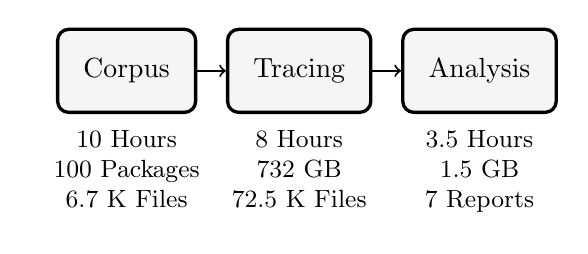
\begin{tikzpicture}
  \definecolor{maroon}{HTML}{D5A6BD}
  \definecolor{darkmaroon}{HTML}{741B47}
  \definecolor{yellow}{HTML}{FFF2CC}
  \definecolor{darkyellow}{HTML}{D6B656}
  \definecolor{blue}{HTML}{DAE8FC}
  \definecolor{darkblue}{HTML}{6C8EBF}
  \definecolor{green}{HTML}{D5E8D4}
  \definecolor{darkgreen}{HTML}{82B366}
  \definecolor{orange}{HTML}{FFE6CC}
  \definecolor{darkorange}{HTML}{D79B00}
  \definecolor{red}{HTML}{F8CECC}
  \definecolor{darkred}{HTML}{B85450}
  \definecolor{purple}{HTML}{E1D5E7}
  \definecolor{darkpurple}{HTML}{9673A6}
  \definecolor{gray}{HTML}{F5F5F5}
  \newcommand{\nodesep}[0]{0.030 \textwidth}
  \newcommand{\textsep}[0]{0.002 \textwidth}
  \newcommand{\backopacity}[0]{0.9}
  \newcommand{\nodename}[1]{\normalsize \begin{tabular}{c}#1\end{tabular}}
  \newcommand{\nodedesc}[1]{\small \begin{tabular}{c}#1\end{tabular}}
  \tikzstyle{block}     = [rectangle, rounded corners, minimum width=.08 \textwidth, minimum height=30pt]
  \tikzstyle{connector} = [line width=0.25mm, ->]

  \node [block, draw = black, very thick, fill = gray]                              (corpus)   {\nodename{Corpus}};
  \node [block, draw = black, very thick, fill = gray, right = \nodesep of corpus]  (tracing)  {\nodename{Tracing}};
  \node [block, draw = black, very thick, fill = gray, right = \nodesep of tracing] (analysis) {\nodename{Analysis}};

  \draw [connector] (corpus)  edge (tracing);
  \draw [connector] (tracing) edge (analysis);

  \node [below = \textsep of corpus]   (corpusdesc)   {\nodedesc{10 Hours\\100 Packages\\6.7 K Files}};
  \node [below = \textsep of tracing]  (tracingdesc)  {\nodedesc{8 Hours\\732 GB\\72.5 K Files}};
  \node [below = \textsep of analysis] (analysisdesc) {\nodedesc{3.5 Hours\\1.5 GB\\7 Reports}};
 \end{tikzpicture}
  \caption{Pipeline}\label{fig:pipeline}
\end{figure}


\paragraph{Corpus} Our corpus is assembled from R packages hosted on CRAN \cite{ligges2017}, the
official R package repository. We mirror CRAN on our server and install its
packages. We downloaded and installed 17,133 CRAN packages.\footnote{Snapshot
taken on 29 May 2021.} From these, we select the 100 CRAN packages with the highest
number of clients. These 100 packages together have 11,786 clients (\ggplot has
the highest number of clients, 2,320, and package \vctrs has the fewest, 108).
These packages contain 481K lines of R code and 1M lines of native code. During
execution, these 100 packages call functions from 186 other packages, so our
evaluation also includes them. These extra packages have 478K lines of R code
and 1.1M lines of native code.

CRAN packages come equipped with runnable code in the form of tests, examples,
and long-form examples called vignettes. Examples demonstrate the use of a
package's functions, and vignettes illustrate a package's functionality with a
larger example, typically using data supplied with the package. These programs
are extracted as independently executable scripts for evaluation by the analysis
pipeline. Overall, there are 6.9K scripts with 205.8K lines of code,
Table~\ref{table:corpus} has details.

\begin{table}[!h]   \small  \centering
  \caption{Corpus}\label{table:corpus}
  \vspace{-3mm}
  \begin{tabular}{lrrr}    \toprule
    &\bf Tests&\bf Examples&\bf Vignettes\\    \midrule
    {Scripts}&1.5K&5.0K&187\\    \midrule
    {LOC}&136.7K&55.2K&13.9K\\
    \bottomrule
  \end{tabular}
\end{table}


\paragraph{Tracing} Execution traces are generated using \envtracer, a dynamic
analyzer built on top of \rdyntrace. \rdyntrace modifies GNU R
4.0.2~\cite{oopsla19b} to record events during program execution. \envtracer
collects execution information associated with environments from these events.

\paragraph{Analysis} The tracing step generates 681GB of data; analyzing data at
this scale is thus the major challenge. We use a custom map-reduce analysis that
first processes individual traces in parallel to generate smaller tables per
program. This is expensive, but it substantially reduces data size. Then the
tables are concatenated into a single table per analysis. Finally, summaries are
computed from the concatenated tables. The report phase generates graphs and
tables from these summaries.


%% \subsection{Dynamic Analysis of R}
%% 
%% Execution traces are generated using \envtracer, a dynamic analyzer built on top
%% of \rdyntrace. \rdyntrace modifies GNU R 4.0.2~\cite{oopsla19b} to record events
%% during program execution. We use these callbacks to collect execution
%% information associated with environments. The events include function entry and
%% exit, eval entry and exit, object allocation and deallocation, package loading
%% and attaching, variable lookup, assignment, and removal, subassignment,
%% subsetting, and attribute setting. When the program exits, \envtracer stores the
%% traces in a tabular format. To handle the subtleties of R, \envtracer maintains
%% models of concrete R objects, such as environments, functions, calls, and frames
%% on the call stack. Model objects have unique identities, whereas R objects are
%% identified by their memory address, and the garbage collector can reuse these.
%% \envtracer heuristically constructs names of model functions. The model stack
%% updates itself appropriately in response to longjump used by R for non-local
%% returns.

\section{How Frequent are Environments?}

The 286 corpus packages have 44K functions, of which 18K are exercised. From the
un-exercised 26K functions, the majority belong to transitively included
packages for which we do not have tests, and, some 8K functions are from our
initial target packages but were unused. Table~\ref{table:packsize} presents the
distribution of exercised functions across these packages. We observe that 171
packages have 25 functions or less. There are few large packages; 8 with more
than 500 functions.

\begin{table}[!h]    \small
  \caption{Package Size} \label{table:packsize}  \centering
  \begin{tabular}{lr}    \toprule
    \bf Functions&\bf Packages\\    \midrule
    1--25&169\\
    26--50&40\\
    51--100&17\\
    101--150&14\\
    151--200&11\\
    201--250&15\\    \bottomrule
  \end{tabular}
  \quad
  \begin{tabular}{lr}    \toprule
    \bf Functions&\bf Packages\\    \midrule
    251--300&4\\
    301--400&6\\
    401--500&2\\
    501--600&3\\
    601--700&0\\
    701--800&3\\    \bottomrule
  \end{tabular}
\end{table}

\noindent
We observed 42M calls to these functions. Figure~\ref{fig:calldist} shows the
distribution of calls: 53\% of functions are called more than ten times, and 14\% of
functions are called only once.

\begin{figure}[!h]
  \centering
  % Created by tikzDevice version 0.12.3.1 on 2021-06-03 17:14:17
% !TEX encoding = UTF-8 Unicode
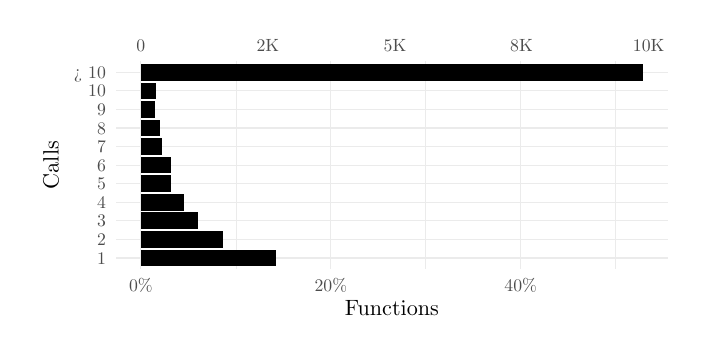
\begin{tikzpicture}[x=1pt,y=1pt]
\definecolor{fillColor}{RGB}{255,255,255}
\path[use as bounding box,fill=fillColor,fill opacity=0.00] (0,0) rectangle (238.49,108.41);
\begin{scope}
\path[clip] ( 31.86, 21.16) rectangle (231.38, 96.31);
\definecolor{drawColor}{gray}{0.92}

\path[draw=drawColor,line width= 0.2pt,line join=round] ( 75.23, 21.16) --
	( 75.23, 96.31);

\path[draw=drawColor,line width= 0.2pt,line join=round] (143.83, 21.16) --
	(143.83, 96.31);

\path[draw=drawColor,line width= 0.2pt,line join=round] (212.43, 21.16) --
	(212.43, 96.31);

\path[draw=drawColor,line width= 0.4pt,line join=round] ( 31.86, 25.19) --
	(231.38, 25.19);

\path[draw=drawColor,line width= 0.4pt,line join=round] ( 31.86, 31.90) --
	(231.38, 31.90);

\path[draw=drawColor,line width= 0.4pt,line join=round] ( 31.86, 38.61) --
	(231.38, 38.61);

\path[draw=drawColor,line width= 0.4pt,line join=round] ( 31.86, 45.32) --
	(231.38, 45.32);

\path[draw=drawColor,line width= 0.4pt,line join=round] ( 31.86, 52.03) --
	(231.38, 52.03);

\path[draw=drawColor,line width= 0.4pt,line join=round] ( 31.86, 58.73) --
	(231.38, 58.73);

\path[draw=drawColor,line width= 0.4pt,line join=round] ( 31.86, 65.44) --
	(231.38, 65.44);

\path[draw=drawColor,line width= 0.4pt,line join=round] ( 31.86, 72.15) --
	(231.38, 72.15);

\path[draw=drawColor,line width= 0.4pt,line join=round] ( 31.86, 78.86) --
	(231.38, 78.86);

\path[draw=drawColor,line width= 0.4pt,line join=round] ( 31.86, 85.57) --
	(231.38, 85.57);

\path[draw=drawColor,line width= 0.4pt,line join=round] ( 31.86, 92.28) --
	(231.38, 92.28);

\path[draw=drawColor,line width= 0.4pt,line join=round] ( 40.93, 21.16) --
	( 40.93, 96.31);

\path[draw=drawColor,line width= 0.4pt,line join=round] (109.53, 21.16) --
	(109.53, 96.31);

\path[draw=drawColor,line width= 0.4pt,line join=round] (178.13, 21.16) --
	(178.13, 96.31);
\definecolor{fillColor}{RGB}{0,0,0}

\path[fill=fillColor] ( 40.93, 89.26) rectangle (222.31, 95.30);

\path[fill=fillColor] ( 40.93, 22.17) rectangle ( 89.89, 28.21);

\path[fill=fillColor] ( 40.93, 28.88) rectangle ( 70.62, 34.92);

\path[fill=fillColor] ( 40.93, 35.59) rectangle ( 61.56, 41.63);

\path[fill=fillColor] ( 40.93, 42.30) rectangle ( 56.31, 48.34);

\path[fill=fillColor] ( 40.93, 55.72) rectangle ( 51.90, 61.75);

\path[fill=fillColor] ( 40.93, 49.01) rectangle ( 51.87, 55.04);

\path[fill=fillColor] ( 40.93, 62.43) rectangle ( 48.49, 68.46);

\path[fill=fillColor] ( 40.93, 69.13) rectangle ( 47.87, 75.17);

\path[fill=fillColor] ( 40.93, 82.55) rectangle ( 46.25, 88.59);

\path[fill=fillColor] ( 40.93, 75.84) rectangle ( 46.18, 81.88);
\end{scope}
\begin{scope}
\path[clip] (  0.00,  0.00) rectangle (238.49,108.41);
\definecolor{drawColor}{gray}{0.30}

\node[text=drawColor,anchor=base,inner sep=0pt, outer sep=0pt, scale=  0.64] at ( 40.85, 99.91) {0};

\node[text=drawColor,anchor=base,inner sep=0pt, outer sep=0pt, scale=  0.64] at ( 86.78, 99.91) {2K};

\node[text=drawColor,anchor=base,inner sep=0pt, outer sep=0pt, scale=  0.64] at (132.72, 99.91) {5K};

\node[text=drawColor,anchor=base,inner sep=0pt, outer sep=0pt, scale=  0.64] at (178.45, 99.91) {8K};

\node[text=drawColor,anchor=base,inner sep=0pt, outer sep=0pt, scale=  0.64] at (224.39, 99.91) {10K};
\end{scope}
\begin{scope}
\path[clip] (  0.00,  0.00) rectangle (238.49,108.41);
\definecolor{drawColor}{gray}{0.30}

\node[text=drawColor,anchor=base east,inner sep=0pt, outer sep=0pt, scale=  0.64] at ( 28.26, 22.98) {1};

\node[text=drawColor,anchor=base east,inner sep=0pt, outer sep=0pt, scale=  0.64] at ( 28.26, 29.69) {2};

\node[text=drawColor,anchor=base east,inner sep=0pt, outer sep=0pt, scale=  0.64] at ( 28.26, 36.40) {3};

\node[text=drawColor,anchor=base east,inner sep=0pt, outer sep=0pt, scale=  0.64] at ( 28.26, 43.11) {4};

\node[text=drawColor,anchor=base east,inner sep=0pt, outer sep=0pt, scale=  0.64] at ( 28.26, 49.82) {5};

\node[text=drawColor,anchor=base east,inner sep=0pt, outer sep=0pt, scale=  0.64] at ( 28.26, 56.53) {6};

\node[text=drawColor,anchor=base east,inner sep=0pt, outer sep=0pt, scale=  0.64] at ( 28.26, 63.24) {7};

\node[text=drawColor,anchor=base east,inner sep=0pt, outer sep=0pt, scale=  0.64] at ( 28.26, 69.95) {8};

\node[text=drawColor,anchor=base east,inner sep=0pt, outer sep=0pt, scale=  0.64] at ( 28.26, 76.66) {9};

\node[text=drawColor,anchor=base east,inner sep=0pt, outer sep=0pt, scale=  0.64] at ( 28.26, 83.37) {10};

\node[text=drawColor,anchor=base east,inner sep=0pt, outer sep=0pt, scale=  0.64] at ( 28.26, 90.08) {> 10};
\end{scope}
\begin{scope}
\path[clip] (  0.00,  0.00) rectangle (238.49,108.41);
\definecolor{drawColor}{gray}{0.30}

\node[text=drawColor,anchor=base,inner sep=0pt, outer sep=0pt, scale=  0.64] at ( 40.93, 13.15) {0{\%}};

\node[text=drawColor,anchor=base,inner sep=0pt, outer sep=0pt, scale=  0.64] at (109.53, 13.15) {20{\%}};

\node[text=drawColor,anchor=base,inner sep=0pt, outer sep=0pt, scale=  0.64] at (178.13, 13.15) {40{\%}};
\end{scope}
\begin{scope}
\path[clip] (  0.00,  0.00) rectangle (238.49,108.41);
\definecolor{drawColor}{RGB}{0,0,0}

\node[text=drawColor,anchor=base,inner sep=0pt, outer sep=0pt, scale=  0.80] at (131.62,  4.40) {Functions};
\end{scope}
\begin{scope}
\path[clip] (  0.00,  0.00) rectangle (238.49,108.41);
\definecolor{drawColor}{RGB}{0,0,0}

\node[text=drawColor,rotate= 90.00,anchor=base,inner sep=0pt, outer sep=0pt, scale=  0.80] at ( 11.20, 58.73) {Calls};
\end{scope}
\end{tikzpicture}

  \caption{Call Distribution}
  \label{fig:calldist}
\end{figure}

\noindent
These functions have a total of 67K parameter positions.
Figure~\ref{fig:paramdist} shows the distribution of parameters: 3\% functions
have none, 22\% have one parameter, and 5\% have over 10. There are 4 functions
with over 50 parameters, and the \texttt{ggplot2::theme} function has 95
parameters.

\begin{figure}[!h]  \centering
  % Created by tikzDevice version 0.12.3.1 on 2021-06-03 17:14:19
% !TEX encoding = UTF-8 Unicode
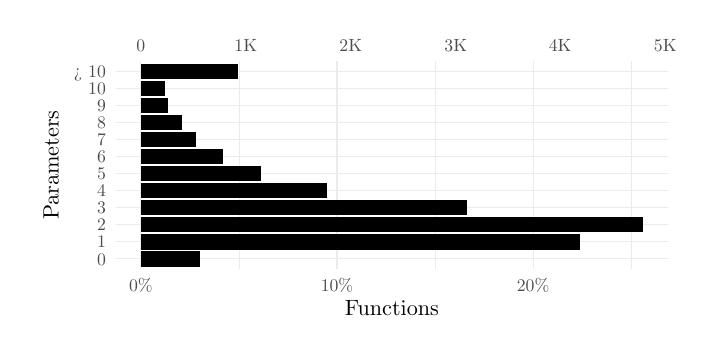
\begin{tikzpicture}[x=1pt,y=1pt]
\definecolor{fillColor}{RGB}{255,255,255}
\path[use as bounding box,fill=fillColor,fill opacity=0.00] (0,0) rectangle (238.49,108.41);
\begin{scope}
\path[clip] ( 31.86, 21.16) rectangle (231.38, 96.31);
\definecolor{drawColor}{gray}{0.92}

\path[draw=drawColor,line width= 0.2pt,line join=round] ( 76.35, 21.16) --
	( 76.35, 96.31);

\path[draw=drawColor,line width= 0.2pt,line join=round] (147.19, 21.16) --
	(147.19, 96.31);

\path[draw=drawColor,line width= 0.2pt,line join=round] (218.04, 21.16) --
	(218.04, 96.31);

\path[draw=drawColor,line width= 0.4pt,line join=round] ( 31.86, 24.86) --
	(231.38, 24.86);

\path[draw=drawColor,line width= 0.4pt,line join=round] ( 31.86, 31.02) --
	(231.38, 31.02);

\path[draw=drawColor,line width= 0.4pt,line join=round] ( 31.86, 37.18) --
	(231.38, 37.18);

\path[draw=drawColor,line width= 0.4pt,line join=round] ( 31.86, 43.34) --
	(231.38, 43.34);

\path[draw=drawColor,line width= 0.4pt,line join=round] ( 31.86, 49.50) --
	(231.38, 49.50);

\path[draw=drawColor,line width= 0.4pt,line join=round] ( 31.86, 55.66) --
	(231.38, 55.66);

\path[draw=drawColor,line width= 0.4pt,line join=round] ( 31.86, 61.81) --
	(231.38, 61.81);

\path[draw=drawColor,line width= 0.4pt,line join=round] ( 31.86, 67.97) --
	(231.38, 67.97);

\path[draw=drawColor,line width= 0.4pt,line join=round] ( 31.86, 74.13) --
	(231.38, 74.13);

\path[draw=drawColor,line width= 0.4pt,line join=round] ( 31.86, 80.29) --
	(231.38, 80.29);

\path[draw=drawColor,line width= 0.4pt,line join=round] ( 31.86, 86.45) --
	(231.38, 86.45);

\path[draw=drawColor,line width= 0.4pt,line join=round] ( 31.86, 92.61) --
	(231.38, 92.61);

\path[draw=drawColor,line width= 0.4pt,line join=round] ( 40.93, 21.16) --
	( 40.93, 96.31);

\path[draw=drawColor,line width= 0.4pt,line join=round] (111.77, 21.16) --
	(111.77, 96.31);

\path[draw=drawColor,line width= 0.4pt,line join=round] (182.62, 21.16) --
	(182.62, 96.31);
\definecolor{fillColor}{RGB}{0,0,0}

\path[fill=fillColor] ( 40.93, 89.84) rectangle ( 76.18, 95.38);

\path[fill=fillColor] ( 40.93, 22.09) rectangle ( 62.34, 27.63);

\path[fill=fillColor] ( 40.93, 28.25) rectangle (199.57, 33.79);

\path[fill=fillColor] ( 40.93, 83.68) rectangle ( 49.80, 89.22);

\path[fill=fillColor] ( 40.93, 34.41) rectangle (222.31, 39.95);

\path[fill=fillColor] ( 40.93, 40.56) rectangle (158.76, 46.11);

\path[fill=fillColor] ( 40.93, 46.72) rectangle (108.20, 52.27);

\path[fill=fillColor] ( 40.93, 52.88) rectangle ( 84.25, 58.43);

\path[fill=fillColor] ( 40.93, 59.04) rectangle ( 70.64, 64.59);

\path[fill=fillColor] ( 40.93, 65.20) rectangle ( 60.94, 70.75);

\path[fill=fillColor] ( 40.93, 71.36) rectangle ( 55.94, 76.91);

\path[fill=fillColor] ( 40.93, 77.52) rectangle ( 50.67, 83.06);
\end{scope}
\begin{scope}
\path[clip] (  0.00,  0.00) rectangle (238.49,108.41);
\definecolor{drawColor}{gray}{0.30}

\node[text=drawColor,anchor=base,inner sep=0pt, outer sep=0pt, scale=  0.64] at ( 40.85, 99.91) {0};

\node[text=drawColor,anchor=base,inner sep=0pt, outer sep=0pt, scale=  0.64] at ( 78.80, 99.91) {1K};

\node[text=drawColor,anchor=base,inner sep=0pt, outer sep=0pt, scale=  0.64] at (116.74, 99.91) {2K};

\node[text=drawColor,anchor=base,inner sep=0pt, outer sep=0pt, scale=  0.64] at (154.69, 99.91) {3K};

\node[text=drawColor,anchor=base,inner sep=0pt, outer sep=0pt, scale=  0.64] at (192.43, 99.91) {4K};

\node[text=drawColor,anchor=base,inner sep=0pt, outer sep=0pt, scale=  0.64] at (230.38, 99.91) {5K};
\end{scope}
\begin{scope}
\path[clip] (  0.00,  0.00) rectangle (238.49,108.41);
\definecolor{drawColor}{gray}{0.30}

\node[text=drawColor,anchor=base east,inner sep=0pt, outer sep=0pt, scale=  0.64] at ( 28.26, 22.65) {0};

\node[text=drawColor,anchor=base east,inner sep=0pt, outer sep=0pt, scale=  0.64] at ( 28.26, 28.81) {1};

\node[text=drawColor,anchor=base east,inner sep=0pt, outer sep=0pt, scale=  0.64] at ( 28.26, 34.97) {2};

\node[text=drawColor,anchor=base east,inner sep=0pt, outer sep=0pt, scale=  0.64] at ( 28.26, 41.13) {3};

\node[text=drawColor,anchor=base east,inner sep=0pt, outer sep=0pt, scale=  0.64] at ( 28.26, 47.29) {4};

\node[text=drawColor,anchor=base east,inner sep=0pt, outer sep=0pt, scale=  0.64] at ( 28.26, 53.45) {5};

\node[text=drawColor,anchor=base east,inner sep=0pt, outer sep=0pt, scale=  0.64] at ( 28.26, 59.61) {6};

\node[text=drawColor,anchor=base east,inner sep=0pt, outer sep=0pt, scale=  0.64] at ( 28.26, 65.77) {7};

\node[text=drawColor,anchor=base east,inner sep=0pt, outer sep=0pt, scale=  0.64] at ( 28.26, 71.93) {8};

\node[text=drawColor,anchor=base east,inner sep=0pt, outer sep=0pt, scale=  0.64] at ( 28.26, 78.09) {9};

\node[text=drawColor,anchor=base east,inner sep=0pt, outer sep=0pt, scale=  0.64] at ( 28.26, 84.25) {10};

\node[text=drawColor,anchor=base east,inner sep=0pt, outer sep=0pt, scale=  0.64] at ( 28.26, 90.41) {> 10};
\end{scope}
\begin{scope}
\path[clip] (  0.00,  0.00) rectangle (238.49,108.41);
\definecolor{drawColor}{gray}{0.30}

\node[text=drawColor,anchor=base,inner sep=0pt, outer sep=0pt, scale=  0.64] at ( 40.93, 13.15) {0{\%}};

\node[text=drawColor,anchor=base,inner sep=0pt, outer sep=0pt, scale=  0.64] at (111.77, 13.15) {10{\%}};

\node[text=drawColor,anchor=base,inner sep=0pt, outer sep=0pt, scale=  0.64] at (182.62, 13.15) {20{\%}};
\end{scope}
\begin{scope}
\path[clip] (  0.00,  0.00) rectangle (238.49,108.41);
\definecolor{drawColor}{RGB}{0,0,0}

\node[text=drawColor,anchor=base,inner sep=0pt, outer sep=0pt, scale=  0.80] at (131.62,  4.40) {Functions};
\end{scope}
\begin{scope}
\path[clip] (  0.00,  0.00) rectangle (238.49,108.41);
\definecolor{drawColor}{RGB}{0,0,0}

\node[text=drawColor,rotate= 90.00,anchor=base,inner sep=0pt, outer sep=0pt, scale=  0.80] at ( 11.20, 58.73) {Parameters};
\end{scope}
\end{tikzpicture}

  \caption{Parameter Distribution}
  \label{fig:paramdist}
\end{figure}

We counted \ObjCntEnvironment environments, which makes them the second most
widely allocated values. Table~\ref{table:object_count_dist} shows the frequency
of other values for comparison. Promises lead as there is one per
parameter~\cite{oopsla19b}. Vectors of logicals and characters are more frequent
than integers, reals, and raw.


\begin{table}[!h]   \small
  \caption{Object Counts} \label{table:object_count_dist}
  \centering
  \begin{tabular}{lr} \toprule
    \textbf{Type}&\textbf{Count}\\\midrule
    Promise&\ObjCntPromise\\
    Environment&\ObjCntEnvironment\\
    Logical&\ObjCntLogical\\
    Character&\ObjCntCharacter\\
    Language&\ObjCntLanguage\\
    Integer&\ObjCntInteger\\\bottomrule
  \end{tabular}
  \begin{tabular}{lr}\toprule
    \textbf{Type}&\textbf{Count}\\\midrule
    List&\ObjCntList\\
    Closure&\ObjCntClosure\\
    Real&\ObjCntReal\\
    Symbol&\ObjCntSymbol\\
    Raw&\ObjCntRaw\\
    Other&\ObjCntOther\\
    \bottomrule
  \end{tabular}
\end{table}

\noindent
Table~\ref{table:api_calls} gives the number of calls made to the various
environment APIs. Each of these functions takes or returns an environment as
an argument. Overall, they cover most of the non-traditional uses of environments.

\begin{table}[!h] \small
  \caption{API Calls} \label{table:api_calls} \centering
  \begin{tabular}{lr}
    \toprule
    \textbf{Function}&\textbf{Calls}\\
    \midrule
    \texttt{substitute}&\CallCntSubstitute\\
    \texttt{environment}&\CallCntEnvironment\\
    \texttt{baseenv}&\CallCntBaseenv\\
    \texttt{as.environment}&\CallCntAsDotenvironment\\
    \texttt{parent.frame}&\CallCntParentDotframe\\
    \texttt{getNamespace}&\CallCntGetnamespace\\
    \texttt{sys.frame}&\CallCntSysDotframe\\
    \texttt{get0}&\CallCntGetZero\\
    \texttt{get}&\CallCntGet\\
    \texttt{sys.parent}&\CallCntSysDotparent\\
    \texttt{[[}&\CallCntDBrack\\
    \bottomrule
  \end{tabular}
  \begin{tabular}{lr}
    \toprule
    \textbf{Function}&\textbf{Calls}\\
    \midrule
    \texttt{sys.function}&\CallCntSysDotfunction\\
    \texttt{list2env}&\CallCntListTwoenv\\
    \texttt{sys.call}&\CallCntSysDotcall\\
    \texttt{parent.env<-}&\CallCntParentDotenvAssign\\
    \texttt{parent.env}&\CallCntParentDotenv\\
    \texttt{\$}&\CallCntDollar\\
    \texttt{.subset2}&\CallCntDotSubsetTwo\\
    \texttt{sys.nframe}&\CallCntSysDotnframe\\
    \texttt{environment<-}&\CallCntEnvironmentAssign\\
    \texttt{\$<-}&\CallCntDollarAssign\\
    \texttt{exists}&\CallCntExists\\
    \bottomrule
  \end{tabular}\\
  \begin{tabular}{lr}
    \toprule
    \textbf{Function}&\textbf{Calls}\\
    \midrule
    \texttt{assign}&\CallCntAssign\\
    \texttt{lockBinding}&\CallCntLockbinding\\
    \texttt{mget}&\CallCntMget\\
    \texttt{emptyenv}&\CallCntEmptyenv\\
    \texttt{as.list}&\CallCntAsDotlist\\
    \texttt{lockEnvironment}&\CallCntLockenvironment\\
    \texttt{globalenv}&\CallCntGlobalenv\\
    \texttt{\~}&\CallCntTilde\\
    \texttt{environmentName}&\CallCntEnvironmentname\\
    \texttt{rm}&\CallCntRm\\
    \bottomrule
  \end{tabular}
  \begin{tabular}{lr}\toprule
    \textbf{Function}&\textbf{Calls}\\\midrule
    \texttt{[[<-}&\CallCntDBrackAssign\\
    \texttt{remove}&\CallCntRemove\\
    \texttt{sys.parents}&\CallCntSysDotparents\\
    \texttt{sys.frames}&\CallCntSysDotframes\\
    \texttt{dynGet}&\CallCntDynget\\
    \texttt{ls}&\CallCntLs\\
    \texttt{unlockBinding}&\CallCntUnlockbinding\\
    \texttt{length}&375\\
    \texttt{objects}& 119\\
    \texttt{pos.to.env}& 7\\\bottomrule
  \end{tabular}
\end{table}

\newpage
\section{Where do Environments come from?}

Table~\ref{table:env_source} presents the distribution of environments by
origin. The \emph{Core} row is for environments created by R's implementation
and its 16 core packages.\footnote{They are base, compiler, {datasets},
{grDevices}, {graphics}, {grid}, {methods}, {parallel}, {profile}, {splines},
{stats}, {stats4}, {tcltk}, {tools}, {translations}, and {utils.}} The
\emph{User} row is for environments that come from user-defined packages. We
further differentiate between environments created in \emph{native} code and in
\emph{R} code. Native environments are created using C APIs: \c{allocSExp},
\c{Rf_NewEnvironment}, and \c{R_NewHashedEnv}. R environments come from calls
to \newEnv. Core is responsible for over 99\% of environments, mostly from C
code. Whereas the 0.03\% of User environment are twice as likely to originate in
R. We encountered 904K environments created during the initialization of the R
session, we ignored those from the rest of the discussion.

\begin{table}[!h]\small\centering
  \caption{Environment Source}\label{table:env_source}
  \begin{tabular}{llrr}\toprule
  &\textbf{Source}&\textbf{\#}&\textbf{\%}\\\midrule
\multirow{2}{*}{\textbf{Core}}&\multicolumn{1}{l}{\emph{Native}}&\multicolumn{1}{r}{1.2B}&\multicolumn{1}{r}{99.62\%}\\
                               & \multicolumn{1}{l}{\emph{R}}     & \multicolumn{1}{r}{3.1M} & \multicolumn{1}{r}{0.27\%}\\\midrule
\multirow{2}{*}{\textbf{User}}  & \multicolumn{1}{l}{\emph{Native}} & \multicolumn{1}{r}{154.9K} & \multicolumn{1}{r}{0.01\%}\\
                                & \multicolumn{1}{l}{\emph{R}}      & \multicolumn{1}{r}{240.4K} & \multicolumn{1}{r}{0.02\%}\\\bottomrule
  \end{tabular}
\end{table}

\noindent
In the Core Native class, 99\% of environments are needed to implement function
environments. There 344K environment used for package namespaces, as well as
2.8M for the S4 object system implemented by the \c{methods} package. Some 165K
were used for \c{eval} and 145K for \c{substitute}. In the Core R class, 94\% of
the environments come from the \c{base} package and 5\% from \c{methods}.


\section{How are Environments Used?}

We divide environments into three categories, presented in
Table~\ref{table:env_category}: \textbf{Calls} are environments used for
evaluating function calls, \textbf{Explicits} are created for non-standard
purposes, and \textbf{Packages} are needed for package loading.

\begin{table}[!h] \small
  \caption{Environment Categories} \label{table:env_category}\centering
  \begin{tabular}{lrr}\toprule
     \textbf{Calls}&     1.2B& 99.3\%\\
    \textbf{Explicits}& 3.7M& 0.3\%\\
    \textbf{Packages}&  3.3M& 0.2\%\\\bottomrule
  \end{tabular}
\end{table}


\subsection{Calls}

Of 1.2B calls, only 20M environments are passed to the functions of
Table~\ref{table:api_calls}. The remaining environments are used only as
``traditional'' environments for creating, reading, and updating variables. To
understand how those 20M environments are used, we summarize manipulation
of these environments with four groups of operations:

\begin{itemize}
\item \texttt{A}: variable reads, writes and removes.
\item \texttt{V}: \eval.
\item \texttt{S}: \substitute.
\item \texttt{X}: \c{parent.frame}, \c{sys.frame} or \c{sys.frames}.
\end{itemize}

\noindent
Any environment may be used by a combination of the operations above.
Table~\ref{table:call_env_seq} has the frequency of the most common ``sets'' of
operations, these are operations that happen to the same environment in no
particular order or frequency. Overall, there are 63 sets but the top four
explain 98\% of non-trivial call environments.

\begin{table}[!h]  \small
  \caption{Operation mix} \label{table:call_env_seq}  \centering
  \begin{tabular}{lrr}    \toprule
    \textbf{Event}&\textbf{\#}&\textbf{Cum. \%}\\\midrule
    \texttt{S}&          9.8M & 46\%\\
    \texttt{X,A}&        8.3M & 86\%\\
    \texttt{X,V,A}&      2.2M & 97\%\\
    \texttt{X,S,V,A}   & 312K & 98\%\\\bottomrule
  \end{tabular}
\end{table}

\begin{itemize}
\item[{\bf S}:] Most uses of \c{substitute} originate from \base package
  functions such as \c{::}. When users write \c{ns::sym}, this has the effect of
  reading variable \c{sym} publicly exported from namespace \c{ns}. Here,
  \substitute is used to access the symbol and namespace names, the names are
  converted to strings, then \c{get} does the actual lookup.

\begin{lstlisting}
`::` <- function(pkg, name) {
  pkg <- as.character(substitute(pkg))
  name <- as.character(substitute(name))
  getExportedValue(pkg, name)
}
\end{lstlisting}\medskip

\item[{\bf X,A}:] These environments are obtained as values and then used for
  accessing their bindings. For instance, \c{register\-S3method::assignWrapped}
  uses \c{parent.frame} to get the caller environment and then evaluates a
  promise in that environment accessing its variables.

\begin{lstlisting}
assignWrapped <- function(x, method, home,
                             envir) {
  method <- method
  home <- home
  delayedAssign(x, get(method, envir = home),
                  assign.env = envir)
}
home <- parent.frame()
assignWrapped(home = home, ...)
\end{lstlisting}\medskip

\item[{\bf X,V,A}:] These environments are obtained for the purpose of
  evaluating code in them. The use of \c{glue::glue} by \c{waldo::path_attr} is
  an example where \c{glue} performs string interpolation by extracting the
  caller's environment and evaluating embedded code blocks.

\begin{lstlisting}
path_attr <- function(path, i) {
  funs <- c("comment", "class", "dim")
  ifelse(i %in% funs,
          glue("{i}({path})"),
          glue("attr({path}, '{i}')"))
}
\end{lstlisting}\medskip

\item[{\bf X,S,V,A}:] These environments are used in a combination of \eval and
  \substitute use cases. This occurs in \c{match.arg} when the set of values
  against which the argument is to be matched are not provided, then
  \c{match.arg} uses \c{substitute} to get argument names and reflectively
  access their default values from the caller environment.

\begin{lstlisting}
match.arg <- function(arg, choices,
                      several.ok = FALSE) {
  sysP <- sys.parent()
  formal.args <- formals(sys.function(sysP))
  argname <- as.character(substitute(arg))
  choices <- eval(formal.args[[argname]], 
                    envir = sys.frame(sysP))
\end{lstlisting}\medskip

\end{itemize}

\noindent
Apart from these, formula construction also stands out as a frequent operation.
These formulas extract the environment of the call in which they are created and
carry them around as attributes. We observed 66K formulas constructed in call
environments. The most common example is the \c{stats::formula} function.

While one could hope an optimizing compiler would optimize most call
environments, unfortunately, there are sufficient number of reflective accesses
that it may be hard for the compiler to be able to determine that an environment
can be elided.

\subsection{Explicits}

Explicit environments created using \newEnv mostly come from core, and 395K are
created in user code.

\subsubsection{Core Explicits}

Nine packages are responsible for all explicits in Core.
Table~\ref{table:core_explicit_pack} shows these packages and the number of
environments created. The \c{base} and \c{methods} packages alone account for
99\% of environments. Table~\ref{table:core_explicit_fun} shows the six
functions that alone contribute to 98\% of all explicit environments.

\begin{table}[!h]
  \small
  \caption{Core Explicit Environment Packages} \label{table:core_explicit_pack}
  \centering
  \begin{tabular}{lrr}
    \toprule
    \textbf{Package}&\textbf{\#}&\textbf{\%}\\
    \midrule
    \c{methods}&3.0M&89.2\%\\
    \c{base}&329.9K&99.0\%\\
    \c{grid}&15.7K&99.5\%\\
    \c{grDevices}&10.7K&99.8\%\\
    \c{stats}&2.7K&99.9\%\\
    \c{compiler}&2.4K&100\%\\
    \c{parallel}&610&100\%\\
    \c{tools}&217&100\%\\
    \c{utils}&7&100\%\\
    \bottomrule
  \end{tabular}
\end{table}


\begin{table}[!h]
  \small
  \caption{Core Explicit Environment Functions} \label{table:core_explicit_fun}
  \centering
  \begin{tabular}{lrr}
    \toprule
    \textbf{Function}&\textbf{\#}&\textbf{Cum. \%}\\
    \midrule
    \c{methods::new}&2.8M&84.3\%\\
    \c{base::eval}&165.5K&89.2\%\\
    \c{base::substitute}&145.8K&93.5\%\\
    \c{methods::.mlistAddToTable}&50.2K&95.0\%\\
    \c{methods::.resetInheritedMethods}&50.2K&96.5\%\\
    \c{methods::makeGeneric}&50.2K&98.0\%\\
    \bottomrule
  \end{tabular}
\end{table}

\noindent
We now turn our attention to how these environments are used.
Table~\ref{table:core_explicit_env_seq} shows the top 5 of the full sets of
operations performed on these environment. These sets include the following new
operations:

\begin{itemize}
\item \texttt{L}: locking environments or bindings.
\item \texttt{Z}: modifying parent environment.
\item \texttt{!}: using environment as parent or lexical scope.
\end{itemize}

\begin{table}[!h]
  \small
  \caption{Core Explicit Environment Events} \label{table:core_explicit_env_seq}
  \centering
  \begin{tabular}{lrr}
    \toprule
    \textbf{Event}&\textbf{\#}&\textbf{Cum. \%}\\
    \midrule
    \texttt{A}&3.0M&88.4\%\\
    \texttt{A,V}&165.6K&93.4\%\\
    \texttt{S}&145.8K&97.7\%\\
    \texttt{A,Z,!}&50.2K&99.2\%\\
    \texttt{A,L,!}&12.1K&99.6\%\\
    \bottomrule
  \end{tabular}
\end{table}

\begin{itemize}
\item[{\bf A}:] This is the most common case; environments that are only used to
  access variables, as in the \c{methods::new} function that is used for
  creating S4 objects.
\item[{\bf A,V}:] These environments are used for evaluation by the \c{eval} and
  \c{evalq} functions.
\item[{\bf S}:] These environments are used with \c{substitute}.
\item[{\bf A,Z,!}:] An example of this is the \c{methods::makeGeneric} function.
  It creates a new environment, assigns the field \c{".Generic"} to the name of
  the generic method, sets its parent as the lexical scope of the function, and
  finally, sets the new environment as the lexical scope of the function.
\begin{lstlisting}
  ev <- new.env()
  parent.env(ev) <- environment(fdef)
  environment(fdef) <- ev
  packageSlot(f) <- package
  assign(".Generic", f, envir = ev)
\end{lstlisting}\medskip

\item[{\bf A,L,!}:] This happens in S4 objects, which lock the object's data
  store.
\end{itemize}

\noindent
Overall, 168K environments are passed to eval, and only 100 were used for
formula construction. Overall, explicit environments are used for evaluation,
substitution, and in the S4 object system. This category is integral to the
language implementation.

\subsubsection{User Explicits}

User explicits come from 55 packages. Table~\ref{table:user_explicit_pack} shows
the distribution of the top 8 packages, which account for 96\% of creations. The
\c{vctrs} package allows for type-coercion and size-recycling of vectors. The
\c{rlang} package provides utility functions for working with objects and a
variant of \c{eval}. The \c{R6} package implements an object-oriented system.
The \c{codetools} package implements code analysis. The \c{ggplot2} package is a
popular plotting library. The \c{testthat} package is used for testing. The
\c{dplyr} package implements a DSL for SQL-like queries on data frames. Lastly,
\c{magrittr} implements the pipe operator for composing function.
Table~\ref{table:user_explicit_fun} shows the top ten functions creating
environments; they contribute to 65\% of all explicits.


\begin{table}[!h]
  \small
  \caption{Explicits Packages} \label{table:user_explicit_pack}
  \centering
  \begin{tabular}{lrr}
    \toprule
    \textbf{Package}&\textbf{\#}&\textbf{Cum. \%}\\
    \midrule
    \c{vctrs}&142.9K&36.2\%\\
    \c{rlang}&75.2K&55.2\%\\
    \c{R6}&74.1K&73.9\%\\
    \c{codetools}&39.2K&83.8\%\\
    \c{ggplot2}&24.3K&90.0\%\\
    \c{testthat}&9.1K&92.3\%\\
    \c{dplyr}&8.3K&94.4\%\\
    \c{magrittr}&6.1K&95.9\%\\
    \bottomrule
  \end{tabular}
\end{table}


\begin{table}[!h]
  \small
  \caption{Explicits Functions} \label{table:user_explicit_fun}
  \centering
  \begin{tabular}{lrr}\toprule
    \textbf{Function}&\textbf{\#}&\textbf{Cum. \%}\\
    \midrule
    \c{R6::generator_funs::new}&63.4K&16.0\%\\
    \c{vctrs::vec_c}&55.7K&30.1\%\\
    \c{codetools::mkHash}&31.3K&38.0\%\\
    \c{ggplot2::ggproto}&24.3K&44.2\%\\
    \c{rlang::eval_tidy}&18.1K&48.8\%\\
    \c{vctrs::vec_slice}&16.5K&52.9\%\\
    \c{rlang::new_data_mask}&13.8K&56.4\%\\
    \c{vctrs::vec_cast_common}&12.8K&59.7\%\\
    \c{vctrs::vec_as_names}&10.7K&62.4\%\\
    \c{R6::create_super_env}&10.6K&65.1\%\\
    \bottomrule
  \end{tabular}
\end{table}


Now, we turn our attention to how these environments are used.
Table~\ref{table:user_explicit_env_seq} shows the top 7 of the 82 operation
mixes which characterize 96\% of these environments. We observe a new operation,
\texttt{@}, used to set class attributes.

\begin{table}[!h]\small
  \caption{Explicits Operations} \label{table:user_explicit_env_seq}
  \centering
  \begin{tabular}{lrr}    \toprule
    \textbf{Events}&\textbf{\#}&\textbf{Cum. \%}\\
    \midrule
    \texttt{A,V}&154.0K&39.0\%\\
    \texttt{A}&102.8K&65.0\%\\
    \texttt{A,!}&43.8K&76.1\%\\
    \texttt{A,@}&38.9K&85.9\%\\
    \texttt{A,L}&30.4K&93.6\%\\
    \texttt{A,L,@}&8.3K&95.7\%\\
    \texttt{A,@,!}&3.2K&96.5\%\\
    \bottomrule
  \end{tabular}
\end{table}

\begin{itemize}
\item[{\bf A,V}:] These environments are created for custom evaluation
  strategies, \ie for evaluating expressions with custom bindings. For example,
  the \c{testthat} library uses them for running tests.

\begin{lstlisting}
test_code <- function(code, env = test_env())  {
  test_env <- new.env(parent = env)
  eval(code, test_env)
\end{lstlisting}\medskip

  \item[{\bf A}:] These environments are used as hash tables and mutable state.
    For example, the \c{codetools::mkHash} function creates an environment to
    store intermediate static analysis information.

\begin{lstlisting}
findGlobals <- function(fun, merge = TRUE) {
  funs <- mkHash()
  enter <- function(v) assign(v, TRUE, funs)
  collectUsage(fun, enterGlobal = enter)
  fnames <- ls(funs, all.names = TRUE)
\end{lstlisting}\medskip

  \item[{\bf A,!}:] These environments are used as parents of other environments
    or functions. For example, the \c{R6} package creates new environments and
    sets them as lexical scope of object methods.

\begin{lstlisting}
assign_func_envs <- function(objs, env) {
  lapply(objs, function(x) {
    if (is.function(x)) environment(x) <- env
    x
  })
}

new <- function(...) {
  env <- new.env(parent=parent_env,hash=FALSE)
  methods <- assign_func_envs(methods, env)
\end{lstlisting}\medskip
  
  \item[{\bf A,@}:] These environments are used to create custom objects which
    can be used for dispatch. For example, the \c{ggproto} objects are explicit
    environments with the \c{"ggproto"} class attribute.

\begin{lstlisting}
ggproto <- function(`_class` = NULL, ...) {
  e <- new.env(parent = emptyenv())
  e$super <- find_super
  class(e) <- c(`_class`, "ggproto", "gg")
\end{lstlisting}\medskip

  \item[{\bf A,L}:] This operation mix is seen in environments created by the R6
    package which locks them during object instantiation to prevent any
    modification.

\begin{lstlisting}
new <- function(...) {
    pub_env <- new.env(parent=emptyenv())
    lockEnvironment(pub_env)
\end{lstlisting}\medskip

  \item[{\bf A,L,@}:] These environments come from the \c{later} package which
    uses them as handles for event loop objects. These objects contain a unique
    loop identifier that is locked to prevent modification. The environments
    are given the class attribute \c{"event_loop"}.

\begin{lstlisting}
create_loop <- function(...) {
loop <- new.env(parent = emptyenv())
class(loop) <- "event_loop"
loop$id <- id
lockBinding("id", loop)
\end{lstlisting}\medskip
  
  \item[{\bf A,@,!}:] These environments shows up in the \c{plyr} package, which
    creates environments with attribute \c{"idf"} for immutable data frames. It
    also assigns getter functions to these environments to access the columns of
    the data frame, and sets their lexical scope to be the environment itself.

\begin{lstlisting}
idata.frame <- function(df) {
  self <- new.env()
  self$`_data` <- df
  self$`_getters` <- lapply(names(df), ...)
  names(self$`_getters`) <- names(df)
  for (name in names(df)) {
    f <- self$`_getters`[[name]]
    environment(f) <- self
  }
  structure(self, class = c("idf"))
}
\end{lstlisting}\medskip
  
\end{itemize}

\noindent
Only 597 environments in this category were used for formula construction. Out
of these, 389 were created in tests. The \c{survival} package stands out as it
creates explicits for formulas. 162K of explicits were used for dynamic code
evaluation. 50K of these environments have a class attribute.
Table~\ref{table:explicit_env_attr} presents the class attributes attached to
environments.

\begin{table}[!h]
  \small
  \caption{Environment Attributes} \label{table:explicit_env_attr}
  \centering
  \begin{tabular}{@{}ll@{}rr@{}}
    \toprule
    \textbf{Package}&\textbf{Attributes}&\textbf{\#}&\textbf{Cum. \%}\\
    \midrule
    \texttt{ggplot2}&\texttt{ggproto gg}&24.3K&47.8\%\\
    \texttt{rlang}&\texttt{rlang\_ctxt\_pronoun}&12.1K&71.5\%\\
    \texttt{R6}&\texttt{R6}&9.2K&89.5\%\\
    \texttt{rlang}&\texttt{r6lite}&3.7K&96.8\%\\
    \texttt{plyr}&\texttt{idf environment}&1.2K&99.2\%\\
    \texttt{later}&\texttt{event\_loop}&279&99.7\%\\
    \texttt{R6}&\texttt{R6ClassGenerator}&113&100\%\\
    \texttt{shiny}&\texttt{session\_proxy}&12&100\%\\
    \texttt{XML}&\texttt{XMLHashTree XMLAbstractDocument}&10.0&100\%\\
    \texttt{xts}&\texttt{replot\_xts environment}&2&100\%\\
    \bottomrule
  \end{tabular}
\end{table}


\subsection{Packages}

We observe 3.3M environments related to packages and namespaces. The package
loading mechanism alone accounts for 2.9M of these. The remaining are used as
package namespaces. 2.3M of these environments originate from
\c{lazyLoadDB\-exec}, an internal function responsible for loading a package's
code from a binary file. A few environments are created internally by the
interpreter to store a package's native functions. The internal structure of
these environments is unspecified.

\section{Enclosing Scope Manipulation}

A closure's enclosing scope can be accessed using \c{env(fun)} and modified
using \c{env(fun)<-e}. Table~\ref{table:encl_scope_api} lists calls to these
functions.

\begin{table}[!h]\small\centering
  \caption{Enclosing Scope API}\label{table:encl_scope_api}  \vspace{-3mm}
  \begin{tabular}{llrrrr}
    \toprule &&\textbf{P\#}&\textbf{F\#}&\textbf{C\#}&\textbf{C\%}\\
    \midrule \multirow{2}{*}{\textbf{environment}}
             & \multicolumn{1}{l}{\emph{Core}} & \multicolumn{1}{r}{\EnvironmentCorePackCnt} & \multicolumn{1}{r}{\EnvironmentCoreFunCnt} & \multicolumn{1}{r}{\EnvironmentCoreCallCnt} & \multicolumn{1}{r}{\EnvironmentCoreCallPerc}\\
             & \multicolumn{1}{l}{\emph{User}} & \multicolumn{1}{r}{\EnvironmentUserPackCnt} & \multicolumn{1}{r}{\EnvironmentUserFunCnt} & \multicolumn{1}{r}{\EnvironmentUserCallCnt} & \multicolumn{1}{r}{\EnvironmentUserCallPerc}\\
    \midrule \multirow{2}{*}{\textbf{environment<-}}
             & \multicolumn{1}{l}{\emph{Core}} & \multicolumn{1}{r}{\EnvAsnCorePackCnt} & \multicolumn{1}{r}{\EnvAsnCoreFunCnt} & \multicolumn{1}{r}{\EnvAsnCoreCallCnt} & \multicolumn{1}{r}{\EnvAsnCoreCallPerc}\\
             & \multicolumn{1}{l}{\emph{User}} & \multicolumn{1}{r}{\EnvAsnUserPackCnt} & \multicolumn{1}{r}{\EnvAsnUserFunCnt} & \multicolumn{1}{r}{\EnvAsnUserCallCnt} & \multicolumn{1}{r}{\EnvAsnUserCallPerc}\\\bottomrule
  \end{tabular}
\end{table}

First, we look at the \c{environment} function called \EnvironmentCoreCallPerc
of the time from Core. The \c{methods::registerS3methods} is responsible for
\EnvironmentBaseRegisterMethodCallPerc of calls to \c{environment}. This function
registers S3 methods for dispatch. It extracts the enclosing environment of the
method and updates the method information in its \c{S3MethodsTable}.

\begin{lstlisting}
defenv <- environment(genfun)
table <- new.env(hash = TRUE, parent = baseenv())
defenv[[".__S3MethodsTable__."]] <- table
\end{lstlisting}\medskip

Overall, the \c{methods} package is responsible for \EnvironmentMethodsCallPerc
of the calls.

The \c{compiler::cmpfun} function, used for byte code compilation
is another client. It extracts the body, formal parameter list, and the
enclosing scope of the function to be compiled.

\begin{lstlisting}
cmpfun <- function (f, options = NULL) {
    cntxt <- make.toplevelContext(makeCenv(environment(f)), options)
    ncntxt <- make.functionContext(cntxt, formals(f), body(f))
\end{lstlisting}\medskip

Only, \EnvironmentUserCallPerc of the calls to \c{environment} originate from
{User}. The primary contributor to these calls is the \c{R.oo} package. This
package implements objects with a \c{getStaticInstance.Class} function that
calls the \c{environment} function.

\begin{lstlisting}
setMethodS3("getStaticInstance", "Class", function(this, ...) {
    environment(static) <- environment(this)
\end{lstlisting}\medskip

We observe that \c{environment<-} is called almost equally by both Core and User
packages. Table~\ref{table:env_asn_callers} gives the top five callers of
\c{environment<-}, which account for \EnvAsnTopFiveCallPerc of calls.

\begin{table}[!h]
  \small
  \centering
  \caption{Top \c{environment<-} Callers}\label{table:env_asn_callers}
  \vspace{-3mm}
  \begin{tabular}{lr}
    \toprule \textbf{Function}&\textbf{Call \%}\\
    \midrule
    \EnvAsnOneCallerName&\EnvAsnOneCallPerc\\
    \EnvAsnTwoCallerName&\EnvAsnTwoCallPerc\\
    \EnvAsnThreeCallerName&\EnvAsnThreeCallPerc\\
    \EnvAsnFourCallerName&\EnvAsnFourCallPerc\\
    \EnvAsnFiveCallerName&\EnvAsnFiveCallPerc\\
    \bottomrule
  \end{tabular}
\end{table}

On the {Core} side, \c{methods}, and \c{stats} are responsible for all calls to
\c{environment<-}. Two functions in \c{methods}, \c{.makeDef\-aultBinding} and
\c{installClassMethod}, are responsible for \EnvAsnMethodsCallPerc of all {Core}
calls.

\begin{lstlisting}
.makeDefaultBinding <- function(...) {
  f <- function(value) ...
  environment(f) <- where
\end{lstlisting}\medskip

The \c{stats::make.link} function returns a list of functions related to
a model. These functions are defined as its inner functions which don't use any
of the parent scope bindings. Before returning, it modifies their definition
environment to be the \c{stats} package namespace.

\begin{lstlisting}
make.link <- function (link)  {
        linkfun <- function(mu) ...
        linkinv <- function(eta) ...
        mu.eta <- function(eta) ...
        valideta <- function(eta) ... 

    environment(linkfun) <- environment(linkinv) <-
    environment(mu.eta) <- environment(valideta) <-
    asNamespace("stats")
\end{lstlisting}\medskip

On the {User} side, \c{R6} dominates calls to \c{environment<-}.
\EnvAsnOneCallerName is the most frequent caller, accounting for half of all
calls. It uses \c{environment<-} to change the enclosing scope of object
methods.

\begin{lstlisting}
assign_func_envs <- function(objs, target_env) {
  lapply(objs, function(x) {
    if (is.function(x)) environment(x) <- target_env
    x
  })
}
\end{lstlisting}\medskip


The \c{MASS::negative.binomial} function uses \c{environment<-} to modify the
parent scope of its inner functions, similar to the \c{stats::make.link}
function described above.

\section{Locking}

Calling \c{lockEnvironment} prevents the introduction of new bindings while
\c{lockBinding} prevents their mutation. Bindings can be unlocked with
\c{unlockEnvironment}; the use of this function triggers a warning from the
automated package checker. Table~\ref{table:lock_unlock_dist} presents the
distribution of calls to these functions.

\begin{table}[!h]
  \small
  \centering
  \caption{Locking and Unlocking API}\label{table:lock_unlock_dist}
  \vspace{-3mm}
  \begin{tabular}{llrrrr}
    \toprule &&\textbf{P\#}&\textbf{F\#}&\textbf{C\#}&\textbf{C\%}\\
    \midrule \multirow{2}{*}{\textbf{lockEnvironment}}
             & \multicolumn{1}{l}{\emph{Core}} & \multicolumn{1}{r}{\LockEnvironmentCorePackCnt} & \multicolumn{1}{r}{\LockEnvironmentCoreFunCnt} & \multicolumn{1}{r}{\LockEnvironmentCoreCallCnt} & \multicolumn{1}{r}{\LockEnvironmentCoreCallPerc}\\
             & \multicolumn{1}{l}{\emph{User}} & \multicolumn{1}{r}{\LockEnvironmentUserPackCnt} & \multicolumn{1}{r}{\LockEnvironmentUserFunCnt} & \multicolumn{1}{r}{\LockEnvironmentUserCallCnt} & \multicolumn{1}{r}{\LockEnvironmentUserCallPerc}\\
    \midrule \multirow{2}{*}{\textbf{lockBinding}}
             & \multicolumn{1}{l}{\emph{Core}} & \multicolumn{1}{r}{\LockBindingCorePackCnt} & \multicolumn{1}{r}{\LockBindingCoreFunCnt} & \multicolumn{1}{r}{\LockBindingCoreCallCnt} & \multicolumn{1}{r}{\LockBindingCoreCallPerc}\\
             & \multicolumn{1}{l}{\emph{User}} & \multicolumn{1}{r}{\LockBindingUserPackCnt} & \multicolumn{1}{r}{\LockBindingUserFunCnt} & \multicolumn{1}{r}{\LockBindingUserCallCnt} & \multicolumn{1}{r}{\LockBindingUserCallPerc}\\
    \midrule \multirow{2}{*}{\textbf{unlockBinding}}
             & \multicolumn{1}{l}{\emph{Core}} & \multicolumn{1}{r}{\UnlockBindingCorePackCnt} & \multicolumn{1}{r}{\UnlockBindingCoreFunCnt} & \multicolumn{1}{r}{\UnlockBindingCoreCallCnt} & \multicolumn{1}{r}{\UnlockBindingCoreCallPerc}\\
             & \multicolumn{1}{l}{\emph{User}} & \multicolumn{1}{r}{\UnlockBindingUserPackCnt} & \multicolumn{1}{r}{\UnlockBindingUserFunCnt} & \multicolumn{1}{r}{\UnlockBindingUserCallCnt} & \multicolumn{1}{r}{\UnlockBindingUserCallPerc}\\
    \bottomrule
  \end{tabular}
\end{table}

\noindent
\c{lockEnvironment} is called \LockEnvironmentCoreCallPerc of the time by three
\c{base} functions, \c{sealNamespace}, \c{attachNamespace}, and \c{envhook}. The
first two initialize package and namespace environments. The third loads code
from a database.

On the {User} side, only packages \c{R6} and \c{rlang} lock environments. Most
calls originate from \c{R6}. An example is the \c{R6::clone} method that locks
the public and private method environments of object clones.

\begin{lstlisting}
clone <- function(deep = FALSE) {
    lockEnvironment(new_1_binding)
    lockEnvironment(new_1_private)
\end{lstlisting}\medskip

The \c{methods} package is responsible for all calls to \c{lockBinding} and
\c{unlockBinding} on the {Core} side. On the {User} side, the use of these
functions is varied. Most package functions call them in a matched pair. For
insance, \c{gtools} locks bindings to circumvent a a bug in
R.\footnote{\url{https://bugs.r-project.org/bugzilla/show_bug.cgi?id=15215}}
Some functions in \c{gtools} cause the bytecode interpreter to run out of stack
space. The package has a function, \c{unByteCodeAssign}, that calls
\c{assignEdgewise} to update the functions that trigger the bug to an equivalent
non-bytecode version.

\begin{lstlisting}
assignEdgewise <- function(name, env, value) {
  unlockBinding(name, env = env)
  assign(name, envir = env, value = value)
  lockBinding(name, env = env)
  invisible(value)
}

unByteCodeAssign <- function(fun) {
  FUN <- unByteCode(fun)
  retval <- assignEdgewise(name=name, env=environment(FUN), value=FUN)
}
\end{lstlisting}\medskip

Overall, \c{R6} is the biggest user of locking. Bindings are rarely unlocked,
and they are never used to inject new bindings in other packages. We only found
one package, \c{data.table}, which unlocked bindings to update base functions
\c{cbind} and \c{rbind}.

%% \section{Call Stack Reflection}
%% 
%% Table~\ref{table:call_stack_ref} gives the distribution of calls to
%% \c{parent.frame}. As usual {Core} is the major user, contributing to
%% \ParentFrameCoreCallPerc of calls. Though, {User} is only
%% \ParentFrameUserCallPerc of calls, there are \ParentFrameUserFunCnt clients of
%% \c{parent.frame} in \ParentFrameUserPackCnt packages.
%% Table~\ref{table:par_frm_top_core_callers} gives the top ten {Core} callers.
%% 
%% \begin{table}[!h]  \small  \centering
%%   \caption{Call Stack Reflection API}\label{table:call_stack_ref} \vspace{-3mm}
%%   \begin{tabular}{llrrrr}
%%     \toprule &&\textbf{P\#}&\textbf{F\#}&\textbf{C\#}&\textbf{C\%}\\
%%     \midrule \multirow{2}{*}{\textbf{parent.frame}}
%%              & \multicolumn{1}{l}{\emph{Core}} & \multicolumn{1}{r}{\ParentFrameCorePackCnt} & \multicolumn{1}{r}{\ParentFrameCoreFunCnt} & \multicolumn{1}{r}{\ParentFrameCoreCallCnt} & \multicolumn{1}{r}{\ParentFrameCoreCallPerc}\\
%%              & \multicolumn{1}{l}{\emph{User}} & \multicolumn{1}{r}{\ParentFrameUserPackCnt} & \multicolumn{1}{r}{\ParentFrameUserFunCnt} & \multicolumn{1}{r}{\ParentFrameUserCallCnt} & \multicolumn{1}{r}{\ParentFrameUserCallPerc}\\ \bottomrule
%%   \end{tabular}
%% \end{table}
%% 
%% 
%% \begin{table}[!h]  \small  \centering
%%   \caption{Top \c{parent.frame} \emph{Core} Callers}\label{table:par_frm_top_core_callers}
%%   \vspace{-3mm}
%%   \begin{tabular}{lr}
%%     \toprule \textbf{Function}&\textbf{Call \%}\\
%%     \midrule
%%     \ParentFrameCoreOneCallerName&\ParentFrameCoreOneCallPerc\\
%%     \ParentFrameCoreTwoCallerName&\ParentFrameCoreTwoCallPerc\\
%%     \ParentFrameCoreThreeCallerName&\ParentFrameCoreThreeCallPerc\\
%%     \ParentFrameCoreFourCallerName&\ParentFrameCoreFourCallPerc\\
%%     \ParentFrameCoreFiveCallerName&\ParentFrameCoreFiveCallPerc\\
%%     \ParentFrameCoreSixCallerName&\ParentFrameCoreSixCallPerc\\
%%     \ParentFrameCoreSevenCallerName&\ParentFrameCoreSevenCallPerc\\
%%     \ParentFrameCoreEightCallerName&\ParentFrameCoreEightCallPerc\\
%%     \ParentFrameCoreNineCallerName&\ParentFrameCoreNineCallPerc\\
%%     \ParentFrameCoreTenCallerName&\ParentFrameCoreTenCallPerc\\
%%     \bottomrule
%%   \end{tabular}
%% \end{table}
%% 
%% \noindent
%% The \c{delayedAssign} is the most frequent client, it uses \c{parent.} \c{frame}
%% to create a promise from an unevaluated expression and bind it to a variable. By
%% default, it uses caller's environment to evaluate the promise. \c{tryCatch}
%% evaluates its argument in the caller's environment. Finally, \c{match.call}
%% reflectively accesses the call expression with all arguments expanded.
%% 
%% 
%% The argument \c{n} to \c{parent.frame} controls the number of frames to go back
%% in the call stack. Passing \c{1} returns the environment of the caller. In our
%% corpus, \c{parent.frame} was called \ParentFrameDepthOneCallPerc of the times
%% with \c{n} as 1. It is invoked with the argument 2 \ParentFrameDepthTwoCallPerc
%% of the time. Finally, \ParentFrameDepthThreeCallPerc of the calls receive the
%% argument {3}.


\section{Conclusion}

This paper looked at first-class environments in R. We introduced the main
functions that operate on environments and reported on an observational study of
100 popular R packages. At the outset, our hope was that we could uncover some
ways to simplify and rationalize the design of R's environments. We conclude
with the rather disappointing observation that it seems that all of the
generality of the environment interface is needed, or at least that it is used.
While in the vast majority of cases environment access could be optimized and
environment could be implemented in a straightforward manner, there are
sufficient number of cases where environments escape and are used in a
reflective manner that it is not clear such optimizations can be widely applied.

\paragraph{Acknowledgments}
This work has received funding from National Science Foundation awards 1759736,
1925644 and 1618732, the Czech Ministry of Education, Youth and Sports from the
Czech Operational Programme Research, Development, and Education, under grant
agreement No. CZ.02.1.01/0.\-0/0.0/15\_003/0000421, and the European Research
Council (ERC) under the European Union’s Horizon 2020 research and innovation
programme, under grant agreement No. 695412.

\bibliography{bib/jv,bib/aviral}

\end{document}
